\section{Elvira Framework}
Elvira is made of 9 packages:
\begin{itemize}
	\item	fusion
	\item	gui
	\item	inference
	\item	localize
	\item	learning
	\item	parser
	\item	potential
	\item	tools
	\item	translator 
\end{itemize}
, inside \verb=learning= package we can find 3 packages:
\begin{itemize}
	\item	classification
	\item	constraints
	\item	preprocessing
\end{itemize}
and also a set of classes.

\verb=preprocessing= package is the proper package to perform preprocessing tasks:
by means of 5 classes as we can see in figure 8.1.
\begin{figure}
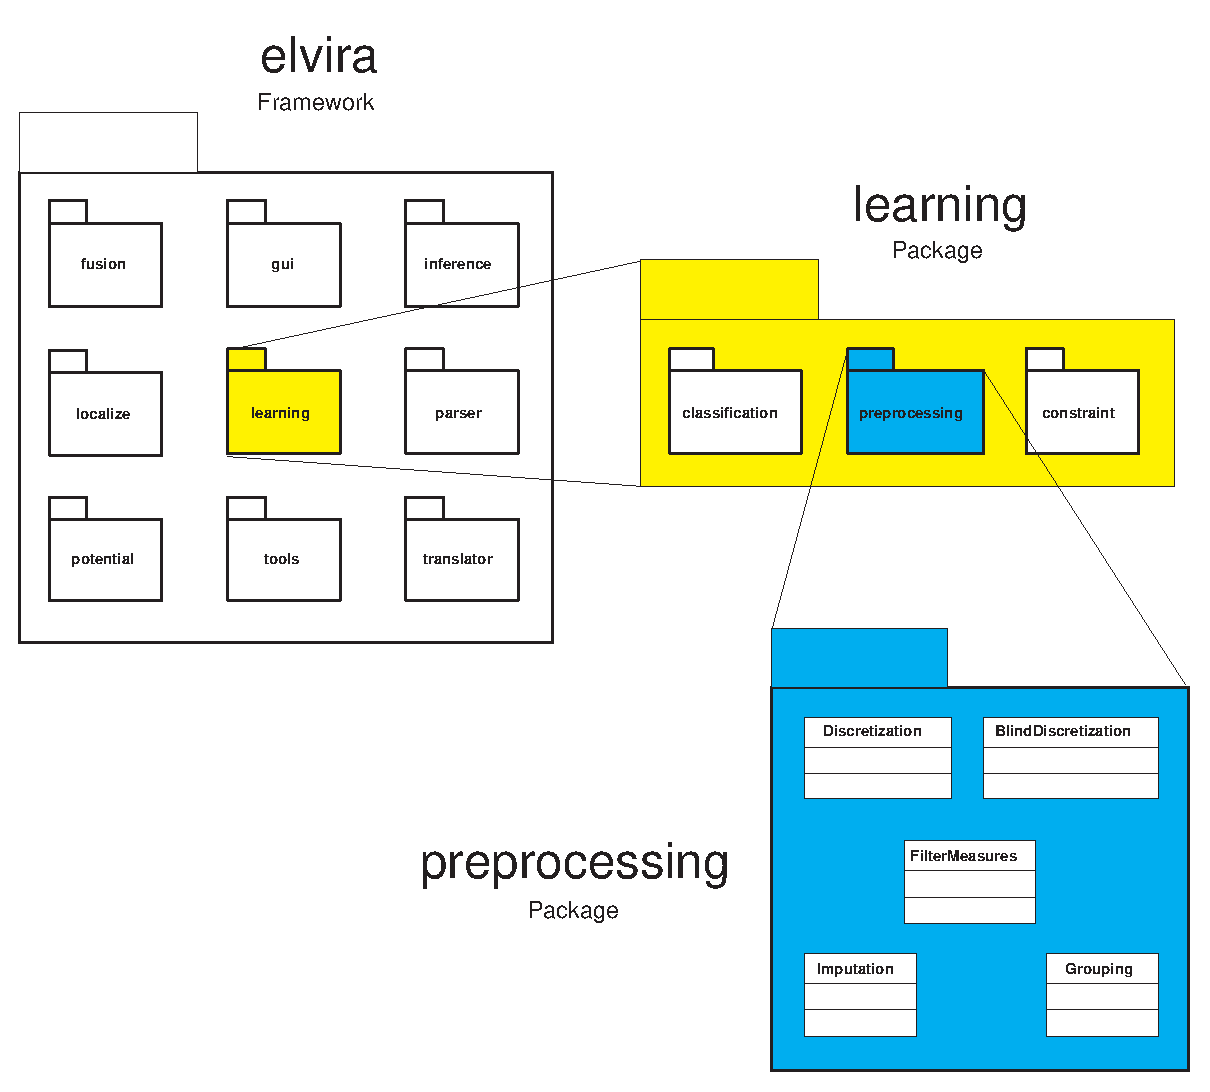
\includegraphics[width=130mm]{Learning/Preprocessing/fig/figure-8.01.eps} 
\label{cap08:01}
\caption{Elvira Framework}
\end{figure}
These are the classes able to perform previously mentioned tasks:
\begin{itemize}
	\item	Filtering Measures: \verb=FilterMeasures.java=
	\item	Discretization: \verb=Discretization.java= and \verb=BlindDiscretization.java=
	\item	Imputation: \verb=Imputation.java=
	\item	Grouping: \verb=Grouping.java=
\end{itemize}

Once \verb=preprocessing= package and the proper set of classes have been located we can proceed
to detail the functioning and the way of using each java class.
